In addition to efforts of technical consortia such as Zigbee, policy makers have also been paying attention to privacy and security issues related to new technologies. From a policy perspective, data security and device security are usually treated as separate issues. Some legislative efforts and policy frameworks are emerging in Europe and the US, but these efforts seem to be still in the early stages. The recent policy efforts have largely focused on the needs of the more mature online ecosystems such as social media platforms. Recently, the newer technologies such as IoT are also gaining attention as these technologies are being utilized in security sensitive settings (such as healthcare or government use).

The purpose of this section is to identify the current regulatory efforts that shape the policy landscape for IoT development. We identified the crucial concepts in IoT security and privacy that we believe can be addressed by policy, and assessed the selected list of regulations in regards to these concepts. This assessment helps identify the areas in which the technical standards can help close the security and privacy gaps vs. the areas where there is need for regulations or new policies to strengthen the IoT ecosystem.

\subsection{Review of Existing Policies}

We restricted our review of the major IoT related privacy and security regulations and standards to those in the US and the EU as these countries tend to share similar values in privacy and have been the leaders in technology regulation. The following table shows the the key principles of device and data security that are addressed in major regulations from these regions that are applicable to home IoT:

%\include{device_sec}
\begin{figure}[h]
	\caption{Device Security}
	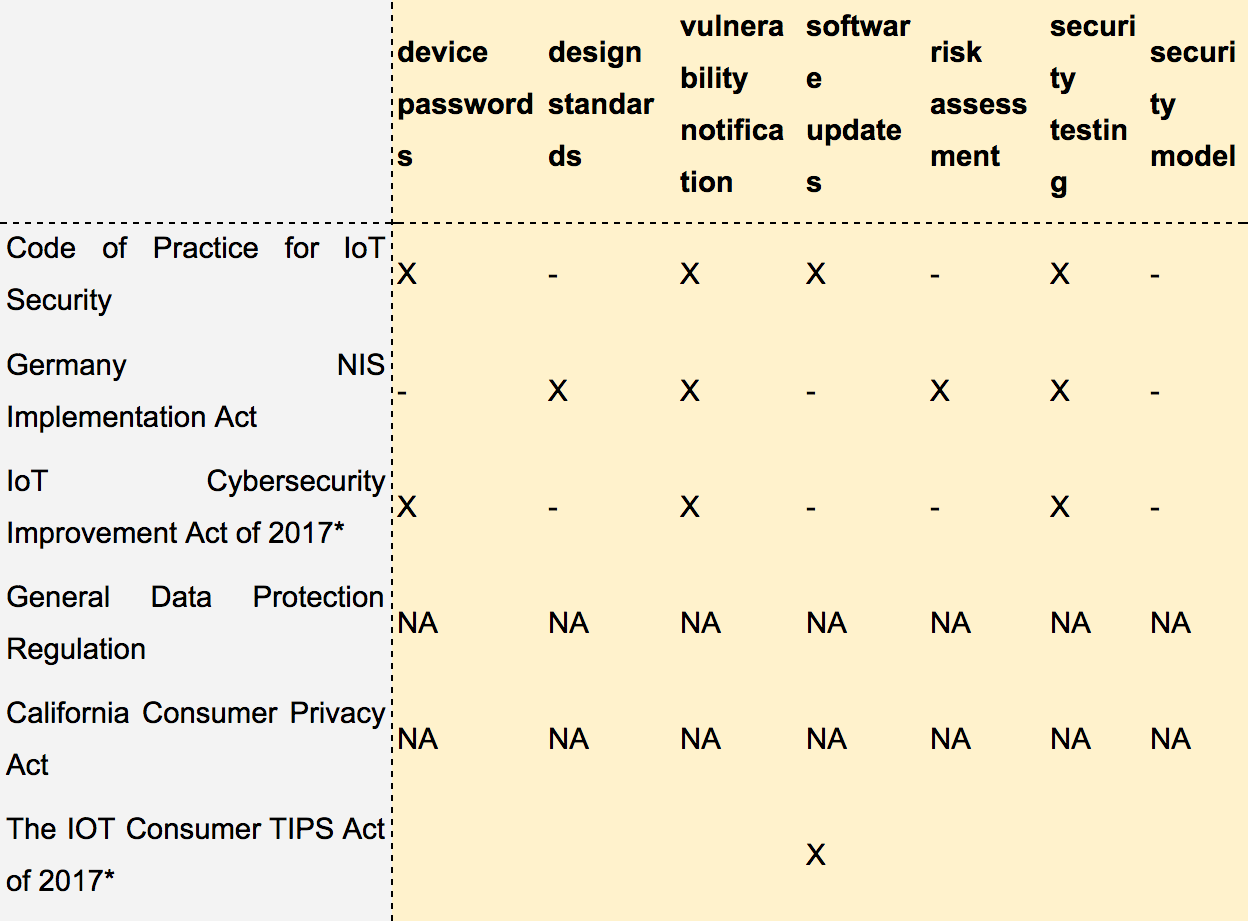
\includegraphics[width=1.0\textwidth]{device}
\end{figure}
%\include{data_sec}
\begin{figure}[h]
	\caption{Data Security}
	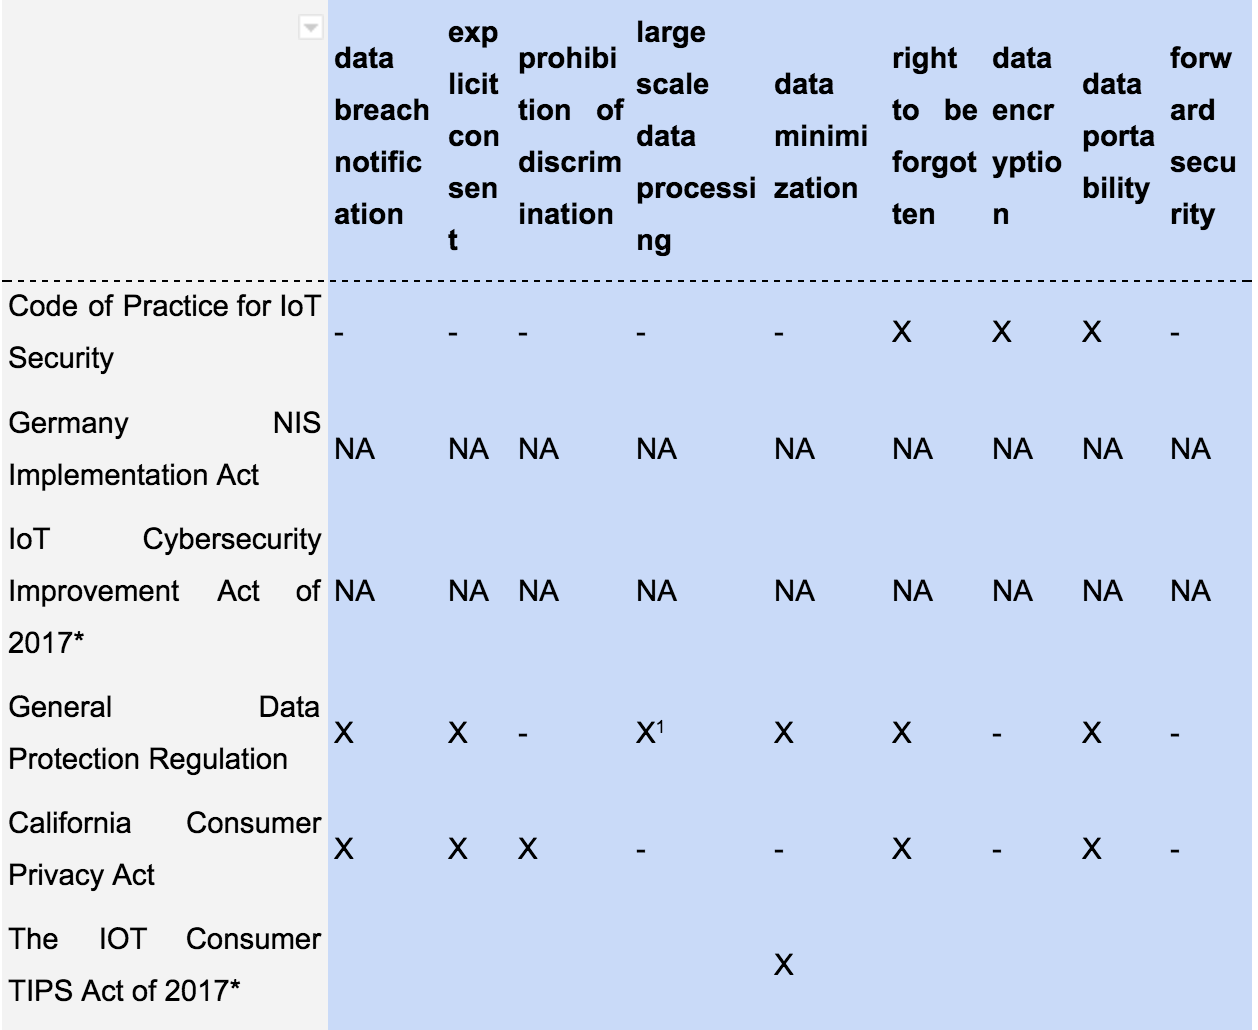
\includegraphics[width=1.0\textwidth]{data}
\end{figure}

Note that the documents marked with * are still in draft form. The IOT Consumer TIPS Act of 2017 and IoT Cybersecurity Improvement Act of 2017 have been introduced, but they await a long process until they pass both the Senate and the House and become a law, and the text may change significantly during the process. For the purposes of our analysis we treated these bills as law of the land in the US, with the assumption that any future law to be implemented by the US government will be largely similar to the present version of these bills.

The range of coverage of these documents vary significantly. While GDPR targets data protection directly, others like the IoT Cybersecurity Improvement Act only focuses on device security questions. The UK’s Code of Practice for IoT Security stands out in the list as the most comprehensive guidelines covering a wide range of topics addressed to many different stakeholders in the IoT ecosystem, but it is currently only a list of recommendations with no liability enforcement on IoT providers.

Looking at the safety and privacy concepts being covered in these policy documents, we observe that some of the concepts such as the right to be forgotten and vulnerability notification are better understood and are addressed by policy makers, while other newer concepts that are more relevant to newer technologies such as IoT are discussed in some or none of the documents. Further discussion of each concept is provided in the next section. 



